\documentclass[pra, onecolumn, notitlepage, floats, 11pt]{revtex4-1}

\usepackage[T1]{fontenc}
\usepackage{graphicx}
\usepackage{color}
\usepackage{latexsym,amsmath}
\usepackage{comment}
\usepackage{tabularx}
\usepackage{siunitx}
\usepackage{multirow}
\usepackage{mathtools}
\usepackage{tikz, fp}
\usepackage{wrapfig}
\usepackage{amsfonts}
\usepackage[pdftex,colorlinks=true, pdfstartview=FitV, linkcolor=linkcolor, citecolor=linkcolor, urlcolor=linkcolor, hyperindex=true,hyperfigures=true]{hyperref} %hyperlink%
\usepackage{fancyhdr}
\usepackage{inconsolata}
\usepackage{listings}
\usepackage{physics}
\usepackage{datetime}
\usepackage[caption=false]{subfig}
\usepackage{titlesec}

\renewcommand{\figurename}{Figure}
\renewcommand{\tablename}{Table}
\renewcommand{\thetable}{\arabic{table}}

\definecolor{airforceblue}{rgb}{0.36, 0.54, 0.66}  %#5D8AA8
\definecolor{cobalt}{rgb}{0.0, 0.28, 0.67}         %#0047AB
\definecolor{coolblack}{rgb}{0.0, 0.18, 0.39}      %#002E63
\definecolor{dartmouthgreen}{rgb}{0.05, 0.5, 0.06} %#00693E
\definecolor{lava}{rgb}{0.81, 0.06, 0.13}          %#CF1020
% move section headings to left
% \sffamily
% \scshape
%\titleformat{\section}{\raggedright\sffamily\bfseries\fontsize{13pt}{13}\selectfont}{\arabic{section}}{1em}{\MakeUppercase}
\titleformat{\section}{\raggedright\bfseries\scshape\fontsize{13pt}{13}\selectfont}{\color{cobalt}\arabic{section}}{1em}{\color{cobalt}}
\titleformat{\subsection}{\raggedright\bfseries\scshape\fontsize{12pt}{12}\selectfont}{{\color{cobalt}\arabic{section}.\arabic{subsection}}}{1em}{\color{cobalt}}
\renewcommand{\thesection}{\arabic{section}}
\renewcommand{\thesubsection}{\arabic{subsection}}
\renewcommand{\thesubsubsection}{\arabic{subsubsection}}
\makeatletter
\renewcommand{\p@subsection}{\thesection.}
\renewcommand{\p@subsubsection}{\thesection.\thesubsection.}
\makeatother


\linespread{0.956}

\DeclarePairedDelimiter\ceil{\lceil}{\rceil}
\DeclarePairedDelimiter\floor{\lfloor}{\rfloor}

\definecolor{linkcolor}{rgb}{0,0,0.65}
\definecolor{shadecolor}{rgb}{0.95, 0.95, 0.95}
\definecolor{mygreen}{rgb}{0,0.6,0}
\definecolor{mygray}{rgb}{0.5,0.5,0.5}
\definecolor{mymauve}{rgb}{0.58,0,0.82}
\lstdefinestyle{fortran}
{
    backgroundcolor=\color{shadecolor},       % background color
    basicstyle=\ttfamily\scriptsize,          % the size of the fonts that are used for the code
    breakatwhitespace=false,                  % sets if automatic breaks should only happen at whitespace
    breaklines=false,                         % sets automatic line breaking
    captionpos=b,                             % sets the caption-position to bottom
    commentstyle=\color{mygreen},             % comment style
    extendedchars=true,                       % lets you use non-ASCII characters; for 8-bits encodings only, does not work with UTF-8
    keepspaces=true,                          % keeps spaces in text, useful for keeping indentation of code (possibly needs columns=flexible)
    keywordstyle=\bfseries\color{blue},       % keyword style
    language=[95]Fortran,                     % the language of the code
    numbers=left,                             % where to put the line-numbers; possible values are (none, left, right)
    numbersep=5pt,                            % how far the line-numbers are from the code
    numberstyle=\tiny\color{mygray},          % the style that is used for the line-numbers
    rulecolor=\color{black},                  % if not set, the frame-color may be changed on line-breaks within not-black text (e.g. comments (green here))
    showspaces=false,                         % show spaces everywhere adding particular underscores; it overrides 'showstringspaces'
    showstringspaces=false,                   % underline spaces within strings only
    showtabs=false,                           % show tabs within strings adding particular underscores
    stepnumber=1,                             % the step between two line-numbers. If it's 1, each line will be numbered
    stringstyle=\color{mymauve},              % string literal style
    tabsize=4,                                % sets default tabsize to 4 spaces
    title=\lstname                            % show the filename of files
}

\lstdefinestyle{python}
{
    backgroundcolor=\color{shadecolor},       % background color
    basicstyle=\ttfamily\scriptsize,          % the size of the fonts that are used for the code
    breakatwhitespace=false,                  % sets if automatic breaks should only happen at whitespace
    breaklines=false,                         % sets automatic line breaking
    captionpos=b,                             % sets the caption-position to bottom
    commentstyle=\color{mygreen},             % comment style
    extendedchars=true,                       % lets you use non-ASCII characters; for 8-bits encodings only, does not work with UTF-8
    keepspaces=true,                          % keeps spaces in text, useful for keeping indentation of code (possibly needs columns=flexible)
    keywordstyle=\bfseries\color{blue},       % keyword style
    language=Python,                          % the language of the code
    numbers=left,                             % where to put the line-numbers; possible values are (none, left, right)
    numbersep=5pt,                            % how far the line-numbers are from the code
    numberstyle=\tiny\color{mygray},          % the style that is used for the line-numbers
    rulecolor=\color{black},                  % if not set, the frame-color may be changed on line-breaks within not-black text (e.g. comments (green here))
    showspaces=false,                         % show spaces everywhere adding particular underscores; it overrides 'showstringspaces'
    showstringspaces=false,                   % underline spaces within strings only
    showtabs=false,                           % show tabs within strings adding particular underscores
    stepnumber=1,                             % the step between two line-numbers. If it's 1, each line will be numbered
    stringstyle=\color{mymauve},              % string literal style
    tabsize=4,                                % sets default tabsize to 4 spaces
    title=\lstname                            % show the filename of files
}

\lstdefinestyle{bash}
{
    backgroundcolor=\color{shadecolor},       % background color
    basicstyle=\ttfamily\scriptsize,          % the size of the fonts that are used for the code
    breakatwhitespace=false,                  % sets if automatic breaks should only happen at whitespace
    breaklines=false,                         % sets automatic line breaking
    captionpos=b,                             % sets the caption-position to bottom
    commentstyle=\color{mygreen},             % comment style
    extendedchars=true,                       % lets you use non-ASCII characters; for 8-bits encodings only, does not work with UTF-8
    keepspaces=true,                          % keeps spaces in text, useful for keeping indentation of code (possibly needs columns=flexible)
    keywordstyle=\bfseries\color{blue},       % keyword style
    language=bash,                            % the language of the code
    numbers=left,                             % where to put the line-numbers; possible values are (none, left, right)
    numbersep=5pt,                            % how far the line-numbers are from the code
    numberstyle=\tiny\color{mygray},          % the style that is used for the line-numbers
    rulecolor=\color{black},                  % if not set, the frame-color may be changed on line-breaks within not-black text (e.g. comments (green here))
    showspaces=false,                         % show spaces everywhere adding particular underscores; it overrides 'showstringspaces'
    showstringspaces=false,                   % underline spaces within strings only
    showtabs=false,                           % show tabs within strings adding particular underscores
    stepnumber=1,                             % the step between two line-numbers. If it's 1, each line will be numbered
    stringstyle=\color{mymauve},              % string literal style
    tabsize=4,                                % sets default tabsize to 4 spaces
    title=\lstname                            % show the filename of files
}


\pagestyle{fancy}
\fancyhf{}
\fancyhead[L]{Rocco Ardino (Mat. 1231629)}
\fancyhead[R]{\bf\thepage}
\fancyfoot[L]{\textsc{report}: Week 7}
\fancyfoot[R]{\today}
\renewcommand{\headrulewidth}{0.1pt}
\renewcommand{\footrulewidth}{0.1pt}

\newcommand{\codebold}[2][cobalt]{\texttt{\bfseries {\color{#1}#2}}}
\newcommand{\code}[2][black]{\color{#1}\texttt{#2}}
\newcommand{\codefunctionbold}[2]{\texttt{\bfseries {\color{cobalt}#1}({\color{lava}#2})}}
\newcommand{\codefunction}[2]{\texttt{#1(#2})}










\begin{document}

\title{Quantum Information and Computing 2020/21\\Week 7 report}

\author{Rocco Ardino}

\date{\today}





\begin{abstract}
    In this work we provide a numerical solution to the time dependent Schr$\mathrm{\ddot{o}}$dinger equation for a monodimensional harmonic oscillator, focusing on the time evolution of the ground state. The split operator method is employed for the purpose and the results found are visualized through a colormap plot, showing the time evolution of the probability wave.
\end{abstract}

\maketitle





\section{Theory}
The time dependent Hamiltonian of the system under study reads:
\begin{equation}
    H(t)
    =
    \underbrace{T}_{\text{kin. term}} + \underbrace{V(t)}_{\text{pot. term}}
    =
    \frac{p^{2}}{2m} + \frac{1}{2} m\omega^{2}\qty[x - x_{0}(t)]^2
    \quad ,
    \label{eq:07_T_1}
\end{equation}
where \( x_{0}(t) = \frac{t}{T} \), with \( T \) a characteristic parameter of the potential. Starting from the work done for the time independent version of last week assignment, we want to solve the time dependent Schr$\mathrm{\ddot{o}}$dinger equation for this type of Hamiltonian in a space interval \( [-a,a] \) and in a time interval \( [t_{0},t_{f}] \).
A good strategy to face the problem is to discretize both space and time intervals into \( N_{x} \) and \( N_{t} \) smaller intervals of width \( \Delta x \) and \( \Delta t \) respectively, defining the steps:
\begin{equation}
    \begin{gathered}
        \begin{aligned}
            x_{i} &= -a + i\Delta x     &   &&   i&=0,\dots,N_{x}  \\
            t_{j} &= t_{0} + j\Delta t  &   &&   j&=0,\dots,N_{t}
        \end{aligned}
    \end{gathered}
    \quad .
    \label{eq:07_T_2}
\end{equation}
Then, we solve the Schr$\mathrm{\ddot{o}}$dinger equation for the starting time \( t_{0} \) through the technique exploited in the previous week assignment. Focusing on the evolution of ground state \( \psi_{0} \) found through diagonalization, we can evolve this state in time through the time evolution operator:
\begin{equation}
    \psi_{0}(x,t_{0}+\Delta t)
    =
    e^{-i\Delta t H} \psi(x,t_{0})
    \quad .
    \label{eq:07_T_3}
\end{equation}
Using te Baker-Campbell-Hausdorff formula and approximating the commutator \( \qty[T,V(t)] \) to zero, we obtain:
\begin{equation}
    e^{-i \Delta t H}
    \approx
    e^{- i \frac{\Delta t}{2} V} e^{- i \Delta t T} e^{- i \frac{\Delta t}{2} V}
    + \mathcal{O}\qty((\Delta t)^3)
    \quad .
    \label{eq:07_T_4}
\end{equation}
It is convenient to apply the operators in the basis where that operator is diagonal. Therefore, the Fourier transform \( \mathcal{F} \) can be employed to switch from the position to the momentum space and viceversa, using \( \mathcal{F}^{-1} \), leading to the main rule of split operator method for the time evolution:
\begin{align}
    \psi_{0}(x_{i+1},t_{j+1})
    &=
    e^{-i \Delta t H(x_{i},t_{j})} \psi (x_{i},t_{j}) \nonumber \\
    &\approx
    e^{- i \frac{\Delta t}{2} V(x_{i},t_{j})}
    A_{\mathcal{F}^{-1}}\mathcal{F}^{-1}
    e^{- i \Delta t T(p_{i})} A_{\mathcal{F}}\mathcal{F}
    e^{- i \frac{\Delta t}{2} V(x_{i},t_{j})}
    \psi_{0}(x_{i},t_{j})
    \quad .
    \label{eq:07_T_5}
\end{align}
with \( A_{\mathcal{F}} = A_{\mathcal{F}^{-1}} = \frac{1}{\sqrt{N_{x}+1}} \) normalization factors of the discrete (anti-)Fourier transform of the wavefunction. This algorthm can be applied iteratively for every time step in order to get the wavefunction solution at time \( t_{f} \).





\section{Code Development}
For this work, the new module \codebold{tdep\_se\_utils} is implemented, containing several functions and subroutines for multiple purposes:
\vspace{-5pt}
\begin{itemize}%[nolistsep]
    \setlength\itemsep{-3pt}
    \item \codefunctionbold{init\_ham}{N,L,M,O,t0,T}, for instantiating the \( (\code{N}+1) \times (\code{N}+1) \) tridiagonal matrix \( H \) with:
    \vspace{-10pt}
    \begin{itemize}
        \setlength\itemsep{-3pt}
        \item[\( \triangleright \)] initial time \code{t0};
        \item[\( \triangleright \)] potential characteristic time parameter \code{T};
        \item[\( \triangleright \)] a symmteric space interval of length \code{L} for the simulation;
        \item[\( \triangleright \)] \code{M} and \code{O} values for the parameters \( m \) and \( \omega \) respectively;
    \end{itemize}
    \vspace{-8pt}
    \item \codefunctionbold{diag\_ham}{ham,eigs}, for diagonalizing the tridiagonal symmetric matrix \code{ham} and returning the eigenvalues and eigenfunctions inside the appropriate input arguments, which are modified during the execution;
    \item \codefunctionbold{ham\_T}{N,L,M}, to get the kinetic term of Hamiltonian;
    \item \codefunctionbold{ham\_V}{N,L,M,O,time,TT}, to get the potential term of Hamiltonian at \( t = \code{time} \);
    \item \codefunctionbold{fft}{psi}, a wrapper to the Fastest Fourier Transform in the West (FFTW3), which returns the FFT of the wavefunction \code{psi};
    \item \codefunctionbold{afft}{psi}, as \code{fft} function but it does the anti-FFT to return in the position space;
    \item \codefunctionbold{time\_ev}{psi,DT,L,M,O,time,TT}, for evolving \code{psi} from \( t_{i} = \code{time} \) to \( t_{i+1} = \code{time} + \code{DT} \);
    \item \codefunctionbold{print\_wvfc}{xs,ys,filename,unit}, for printing on a certain file real and imaginary part of the discretized wavefunction \( \psi \) at a certain time step;
    \item \codefunctionbold{print\_wvfc\_cmap}{xs,ys,zs,filename,unit}, for printing on a certain file the discretized squared modulus \( \abs{\psi(x_{i},t_{i})}^2 \) for every point of the space grid and for every time step, in order to get a file for colormap plot;
    \item \codefunctionbold{print\_wvfc\_expv}{xs,ys,zs,filename,unit}, for printing on a certain file the expectation value \( \expval{x} \) for every time step.
\end{itemize}

Moreover, another module, namely \codebold{cmdline}, is implemented to have a command-line argument parser and for default arguments handling. In particular, we explain the new core functionalities of both the modules in the following subsections.



\subsection{(Anti-)Fast Fourier Transform wrapper}
The code to perform the discrete FFT of the wave function is showed in Listing \ref{lst:07_C_SS_1_1}. This is nothing more than a wrapper of the \codebold[black]{fftw3} functions for FFT, for which a plan is usually defined, then executed and finally destroyed.

%\medskip
\begin{lstlisting}[
    style=fortran,
    frame=single,
    label={lst:07_C_SS_1_1},
    caption={Implementation of the wrapper of \code{fftw3} FFT functions.}
]
function fft(psi) result(FFT_psi)
    ! input arguments
    complex(8), dimension(:) :: psi

    complex(8), dimension(size(psi,1)) :: FFT_psi
    integer(4) :: N
    integer(8) :: plan

    N = size(psi,1)

    call dfftw_plan_dft_1d(plan, N, psi, FFT_psi, -1, 64)
    call dfftw_execute_dft(plan, psi, FFT_psi)
    call dfftw_destroy_plan(plan)
end function fft
\end{lstlisting}

On the other side, the code to perform the discrete anti-FFT (AFFT), and so to return the wavefunction in position space, is showed in Listing \ref{lst:07_C_SS_1_2}. The implementation is analogous to the one written for FFT wrapper.

%\medskip
\begin{lstlisting}[
    style=fortran,
    frame=single,
    label={lst:07_C_SS_1_2},
    caption={Implementation of the wrapper of \code{fftw3} AFFT functions.}
]
function afft(psi) result(AFFT_psi)
    ! input arguments
    complex(8), dimension(:) :: psi

    complex(8), dimension(size(psi,1)) :: AFFT_psi
    integer(4) :: N
    integer(8) :: plan

    N = size(psi,1)

    call dfftw_plan_dft_1d(plan, N, psi, AFFT_psi, +1, 64)
    call dfftw_execute_dft(plan, psi, AFFT_psi)
    call dfftw_destroy_plan(plan)
end function afft
\end{lstlisting}



\subsection{Time evolution through Split Operator Method}
The wrappers previously described are called inside the subroutine \codebold[black]{time\_ev}. The latter evolves the input vector, namely the wave function, of a time step \( \Delta t \), keeping track of the actual time of simulation and of the other parameters of the Hamiltonian in order to reconstruct the kinetic and potential terms. The implementation of the subroutine is showed in Listing \ref{lst:07_C_SS_2_1}.

%\medskip
\begin{lstlisting}[
    style=fortran,
    frame=single,
    label={lst:07_C_SS_2_1},
    caption={Implementation of the subroutine for time evolution of \( \psi \) at a time \( t \) and of a step \( \Delta t \).}
]
subroutine time_ev(psi, DT, L, M, O, time, TT)
    ! input arguments
    complex(8), dimension(:) :: psi
    real(8) :: DT, time, TT
    real(8) :: L, M, O

    real(8), dimension(size(psi,1)) :: V
    real(8), dimension(size(psi,1)) :: T
    integer(4) :: N
    integer(4) :: ii

    N = size(psi,1) - 1

    V = ham_V(N, L, M, O, time, TT)     ! potential term
    T = ham_T(N, L, M)                  ! kinetic   term

    ! apply exponential containing the potential term
    do ii=1,N+1
        psi(ii) = ZEXP(COMPLEX(0.0d0,-0.5d0*DT*V(ii))) * psi(ii)
    end do
    ! fft of wave function and normalization
    psi = fft(psi) / SQRT(1.0d0*N+1)
    ! apply exponential containing the kinetic term
    do ii=1,N+1
        psi(ii) = ZEXP(COMPLEX(0.0d0,-1.0d0*DT*T(ii))) * psi(ii)
    end do
    ! afft of wave function and normalization
    psi = afft(psi) / SQRT(1.0d0*N+1)
    ! apply exponential containing the potential term
    do ii=1,N+1
        psi(ii) = ZEXP(COMPLEX(0.0d0,-0.5d0*DT*V(ii))) * psi(ii)
    end do
end subroutine time_ev
\end{lstlisting}



\subsection{Main program}
Lastly, all the functions described before are employed in a main program, in which a command-line argument parser is implemented in order to obtain an easier handling of the parameters of the simulation. Moreover, this functionality is also capable of giving default values to the arguments when they are not given.
To make the program more user-friendly a \code{-h} help option has been added and in the beginning of the execution all the arguments given are printed along with a flag: \codebold[red]{F} if a value is given for it, \codebold[dartmouthgreen]{T} if default is taken. An example of this functionality and of the way to start the program is showed in Listing \ref{lst:07_C_SS_3_1}. A complete list of the options is given in Table \ref{tab:07_C_SS_3_1}.

\begin{table}[!h]
\begin{minipage}[t]{0.48\textwidth}
    \raisebox{-\height}{
    {\footnotesize
    \begin{tabular}{cccc}
        \toprule
        Arg option    &   Arg name        &   Arg meaning   &   Default     \\
        \colrule
        \code{-NX}    &   \code{stepsX}   &   \( N_{x} \)   &   \( 1000 \)  \\
        \code{-L}     &   \code{lengthX}  &   \( L \)       &   \( 10 \)    \\
        \code{-NT}    &   \code{stepsT}   &   \( N_{t} \)   &   \( 1000 \)  \\
        \code{-T}     &   \code{lengthT}  &   \( T \)       &   \( 5 \)     \\
        \code{-TF}    &   \code{finalT}   &   \( t_{f} \)   &   \( 5 \)     \\
        \code{-M}     &   \code{mass}     &   \( m \)       &   \( 1 \)     \\
        \code{-O}     &   \code{omega}    &   \( \omega \)  &   \( 1 \)     \\
        \code{-h}     &   \code{help}     &   print help    &               \\
        \botrule
    \end{tabular}
    }}
    \caption{Command-line arguments of the program.}
    \label{tab:07_C_SS_3_1}
\end{minipage}
\hfill
\begin{minipage}[t]{0.48\textwidth}
\begin{lstlisting}[
    style=bash,
    frame=single,
    escapechar=!,
    label={lst:07_C_SS_3_1},
    caption={Example of launch and user interface.}
]
!{\bfseries\color{dartmouthgreen}\$}! !{\bfseries\color{cobalt}./07.o}! !{\bfseries\color{lava}-NX}! 2000 !{\bfseries\color{lava}-NT}! 2000 !{\bfseries\color{lava}-T}! 1 !{\bfseries\color{lava}-TF}! 8

Running with the following cmdline options:

NX =	    2000	default [T/F]: !{\bfseries\color{red}F}!
L  =	 10.    	default [T/F]: !{\bfseries\color{dartmouthgreen}T}!
NT =	    2000	default [T/F]: !{\bfseries\color{red}F}!
T  =	 1.0    	default [T/F]: !{\bfseries\color{red}F}!
TF =	 8.0    	default [T/F]: !{\bfseries\color{red}F}!
M  =	 1.0    	default [T/F]: !{\bfseries\color{dartmouthgreen}T}!
O  =	 1.0    	default [T/F]: !{\bfseries\color{dartmouthgreen}T}!
\end{lstlisting}
\end{minipage}
\end{table}

After the parser, if no exceptions are found, a subroutine with the simulation is called, storing \( \operatorname{Re}[\psi(x,t_{j})] \) and \( \operatorname{Im}[\psi(x,t_{j})] \) for the \( j^{\text{th}} \) time step in the dedicated folder \code{results} in the format ``\code{i}\_step\_wvfc.dat''. This is done for every \( j = 0, \dots, N_{t} \).
Moreover, a bigger file ``cmap\_wvfc.dat'' containing all the \( \abs{\psi (x_{i},t_{j})}^{2} \) for every \( i,j \) is saved to produce a colormap plot to visualize both space and time evolution.

Last but not least, the program must be compiled with the flag \code{-ffree-line-length-0} and linking the lapack and fftw3 libraries.





\section{Results}
The simulation is run for \( N_{x} = N_{t} = 2000 \), \( L = 20 \). The characteristic time \( T \) of the potential is set to the default value of \( 1 \), while \( t_{0} \) and \( t_{f} \) are set to \( 0 \) and \( 8 \) respectively. Several values of the physical parameters \( (m, \omega) \) are tested.
The results for the evolution of \( \abs{\psi(x,t)}^{2} \) are showed for all the sets of \( (m, \omega) \) in Figures \ref{fig:07_R_12}, \ref{fig:07_R_34}, \ref{fig:07_R_56} and \ref{fig:07_R_78}. In all the cases, the main point to observe is that the expectation value for the position, namely \( \expval{x} \), evolves with constant velocity towards the right side of the box, with a small sinusoidal component of oscillation. This is the behaviour expected from the given Hamiltonian with such potential.

\begin{figure*}[!h]
    \centering
    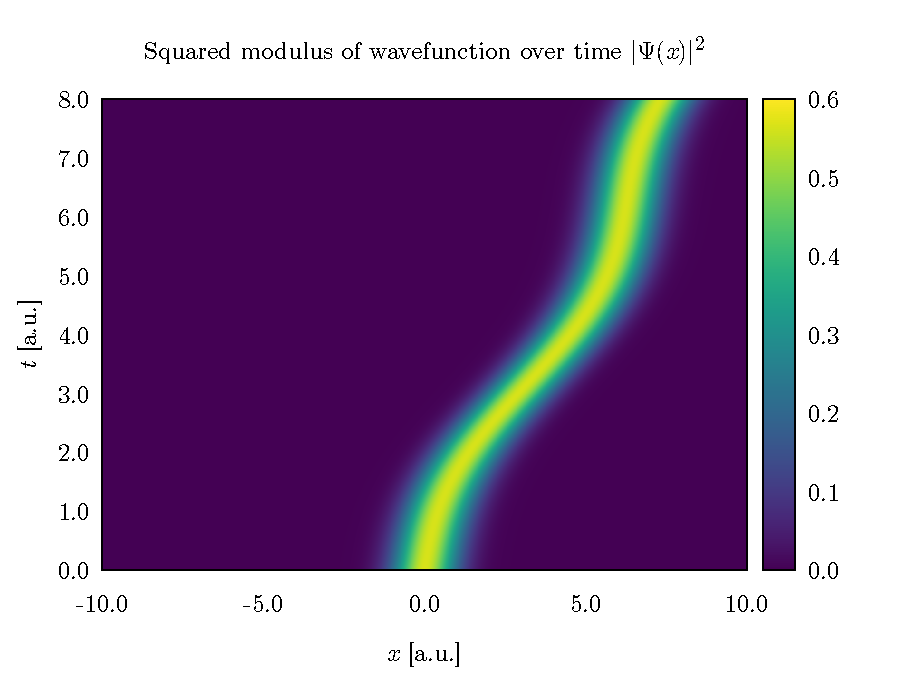
\includegraphics[width=0.40\textwidth]{images/cmap_1_M_1_O.pdf}
    \hspace{1cm}
    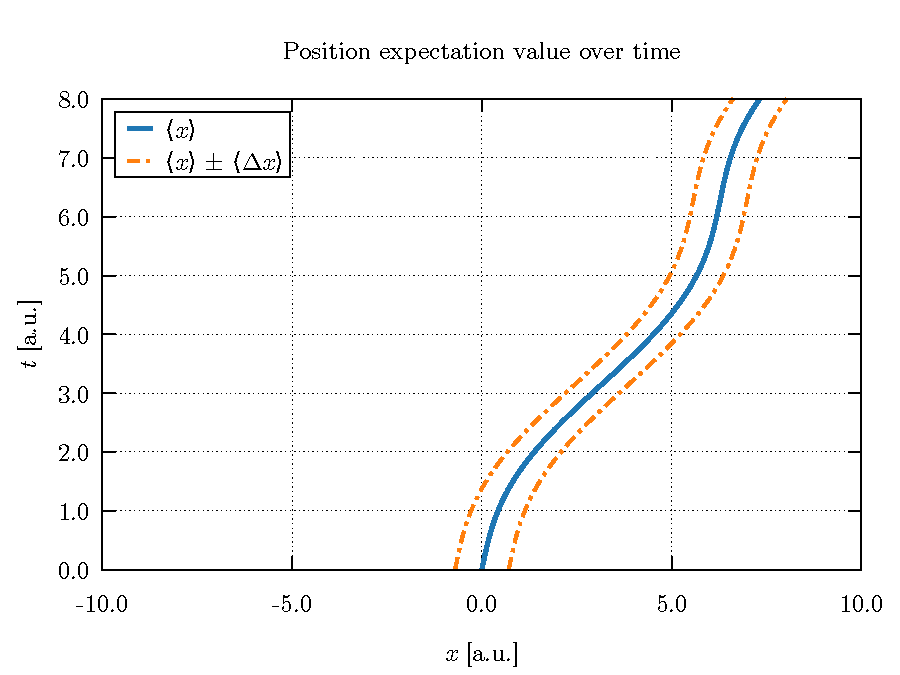
\includegraphics[width=0.40\textwidth]{images/expv_1_M_1_O.pdf}
    \caption{\( (m,\omega) = (1,1) \): colormap and \( \expval{x} \) evolution of the probability wave \( \abs{\psi(x,t)}^{2} \).}
    \label{fig:07_R_12}
\end{figure*}
\begin{figure*}[!h]
    \centering
    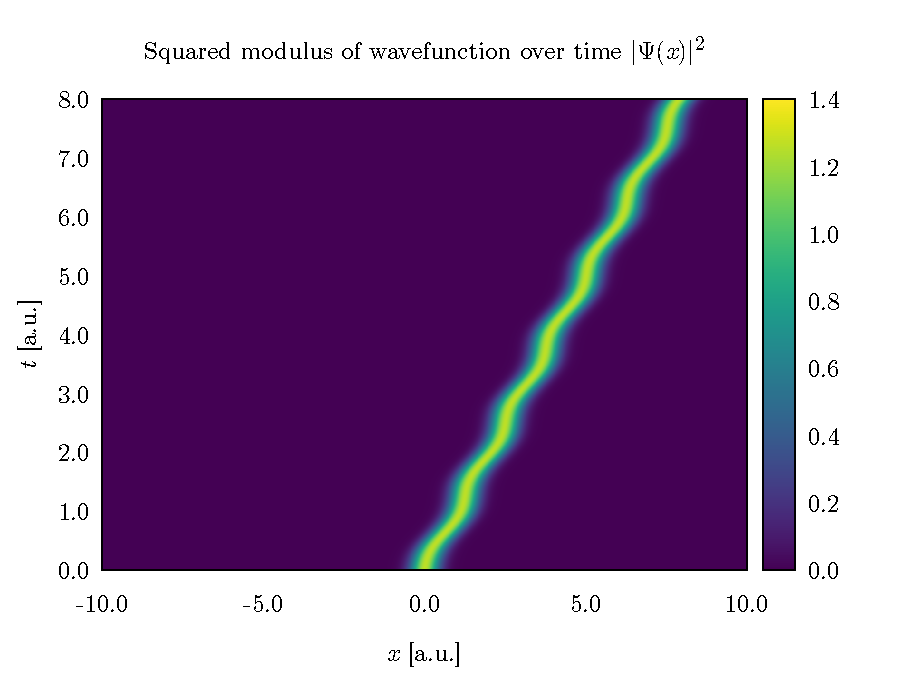
\includegraphics[width=0.40\textwidth]{images/cmap_1_M_5_O.pdf}
    \hspace{1cm}
    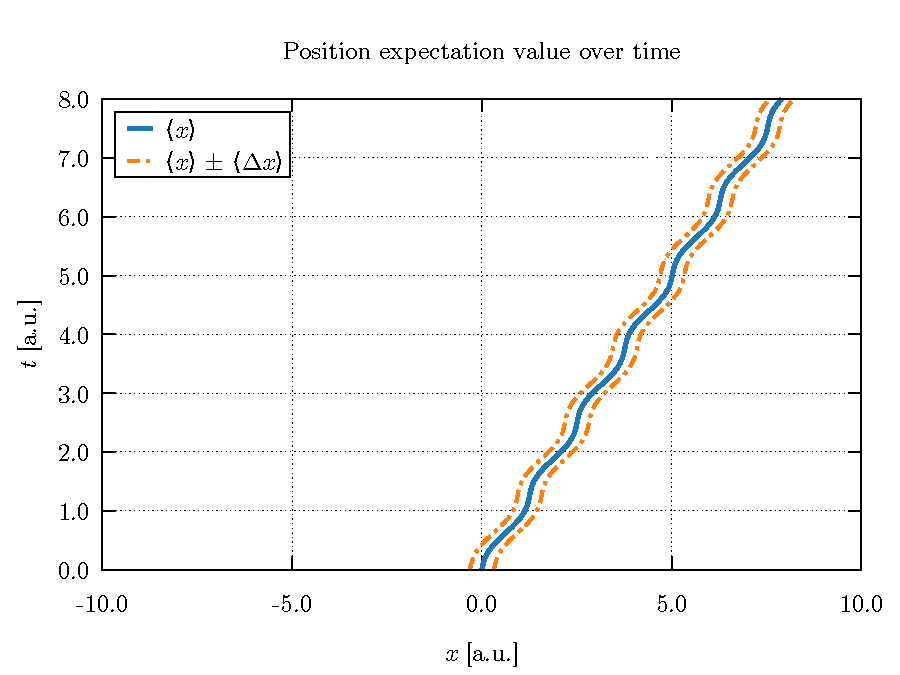
\includegraphics[width=0.40\textwidth]{images/expv_1_M_5_O.pdf}
    \caption{\( (m,\omega) = (1,5) \): colormap and \( \expval{x} \) evolution of the probability wave \( \abs{\psi(x,t)}^{2} \).}
    \label{fig:07_R_34}
\end{figure*}
\begin{figure*}[!h]
    \centering
    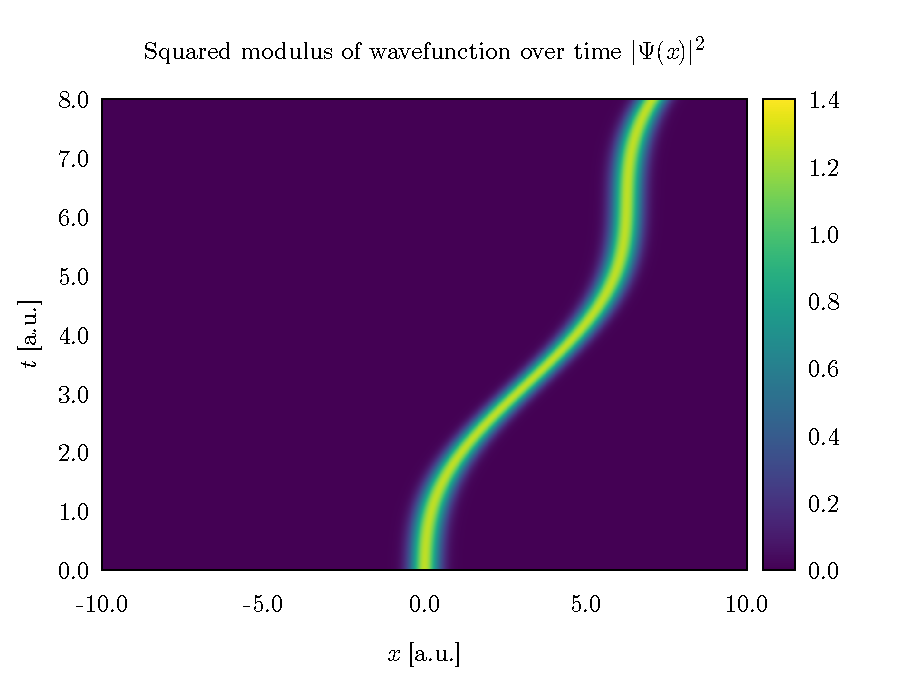
\includegraphics[width=0.40\textwidth]{images/cmap_5_M_1_O.pdf}
    \hspace{1cm}
    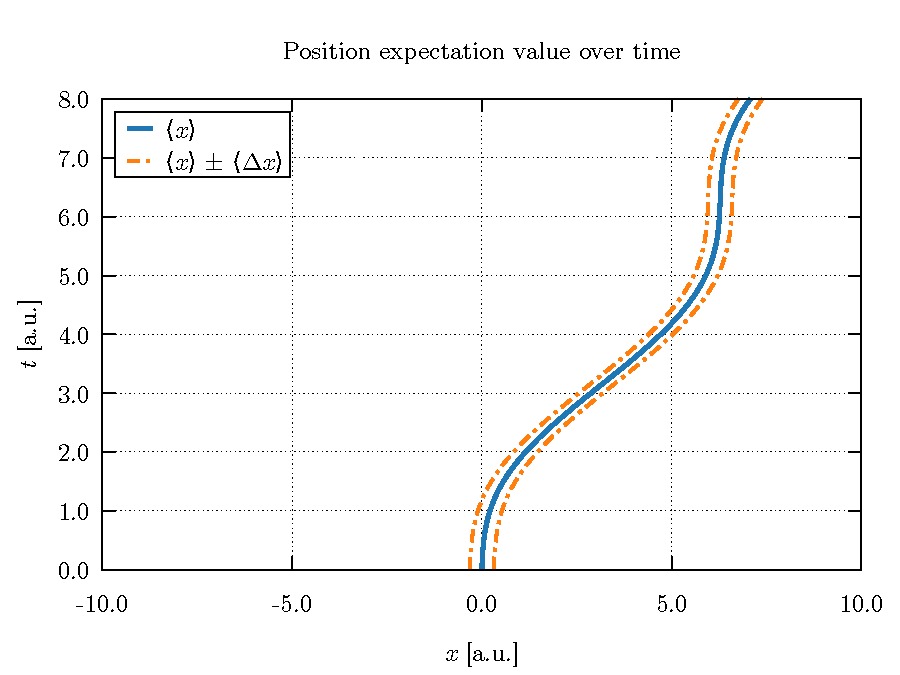
\includegraphics[width=0.40\textwidth]{images/expv_5_M_1_O.pdf}
    \caption{\( (m,\omega) = (5,1) \): colormap and \( \expval{x} \) evolution of the probability wave \( \abs{\psi(x,t)}^{2} \).}
    \label{fig:07_R_56}
\end{figure*}
\begin{figure*}[!h]
    \centering
    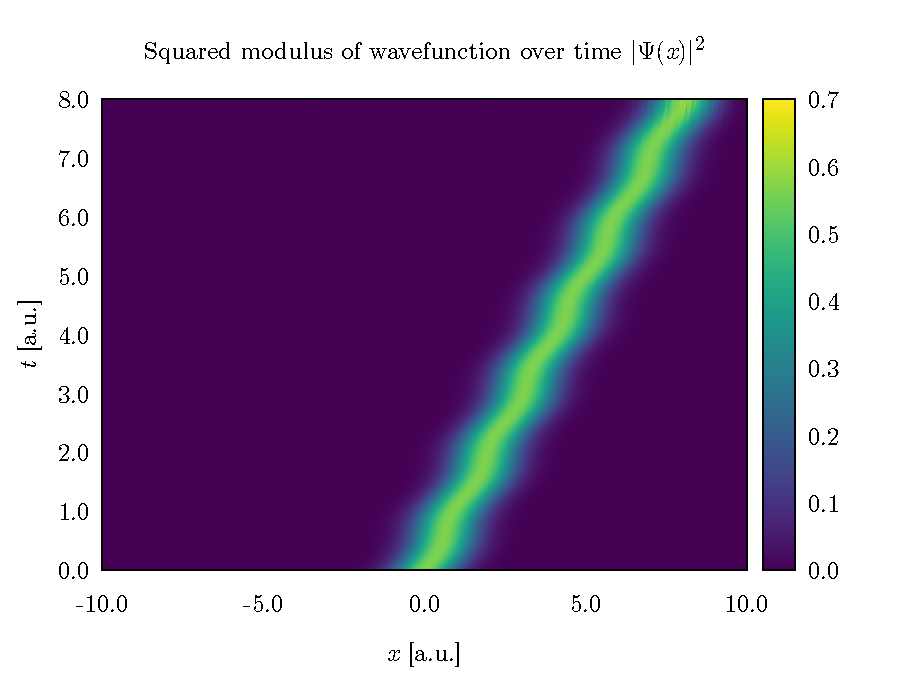
\includegraphics[width=0.40\textwidth]{images/cmap_0.2_M_5_O.pdf}
    \hspace{1cm}
    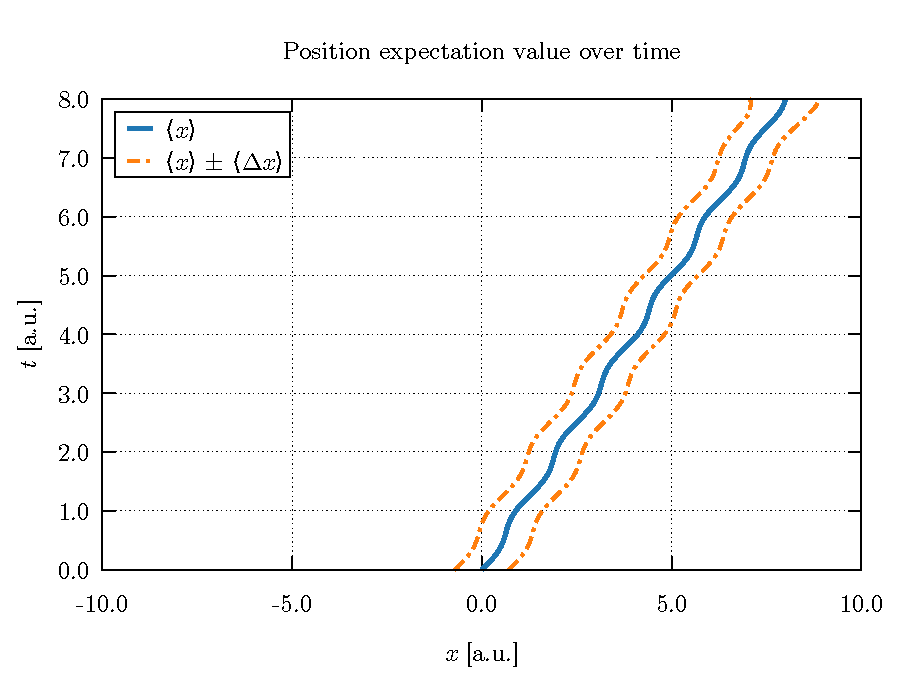
\includegraphics[width=0.40\textwidth]{images/expv_0.2_M_5_O.pdf}
    \caption{\( (m,\omega) = (0.2,5) \): colormap and \( \expval{x} \) evolution of the probability wave \( \abs{\psi(x,t)}^{2} \).}
    \label{fig:07_R_78}
\end{figure*}




\section{Self-evaluation}
The numerical simulation of the time dependent Schr$\mathrm{\ddot{o}}$dinger equation has led to successful results. We managed to work with both Lapack and FFTW3 libraries and to observe the evolution of the ground state of the given Hamiltonian, confirming the correctness of the code written. The implementation was done in a user-friendly and accurate way, introducing also an argument parser with a help functionality in order to understand the needed parameters for the simulation and their meanings.

\end{document}
